\section{Định nghĩa và Phạm vi}
\label{sec:definition_and_scope}

\subsection{Giới thiệu: Bài toán Nghịch đảo và Nỗ lực Diễn giải Thế giới}

Thị giác Máy tính (Computer Vision - CV) là một lĩnh vực khoa học và công nghệ với mục tiêu xây dựng các hệ thống nhân tạo có khả năng thu nhận, xử lý, phân tích, và diễn giải thông tin từ thế giới thị giác. Cốt lõi của nó là một nỗ lực nhằm tự động hóa và tái tạo các năng lực của hệ thống thị giác con người. Trong tác phẩm kinh điển "Vision" \cite{Marr1982}, David Marr đã định nghĩa thị giác là quá trình "biết cái gì đang ở đâu bằng cách nhìn". Định nghĩa tưởng chừng đơn giản này ẩn chứa một thách thức khổng lồ, bởi nó thực chất là một \textbf{bài toán nghịch đảo (inverse problem)}.

Thế giới vật lý của chúng ta là ba chiều (3D), phức tạp, và chứa đựng vô số thông tin về hình dạng, vật liệu, ánh sáng. Quá trình một chiếc máy ảnh (hay mắt người) tạo ra một bức ảnh là một quá trình "thuận": nó chiếu một thế giới 3D phức tạp xuống một mặt phẳng 2D, làm mất đi vô số thông tin (đặc biệt là thông tin về chiều sâu). Bài toán của Thị giác Máy tính là "nghịch đảo" quá trình này: từ một hoặc nhiều hình ảnh 2D thiếu thông tin, chúng ta phải suy luận ngược lại để tái tạo và hiểu được cấu trúc 3D và các thuộc tính ngữ nghĩa của thế giới đã tạo ra chúng. Đây là một bài toán "ill-posed" (bài toán đặt không chỉnh) vì một hình ảnh 2D có thể được tạo ra bởi vô số cảnh 3D khác nhau.

\begin{center}
    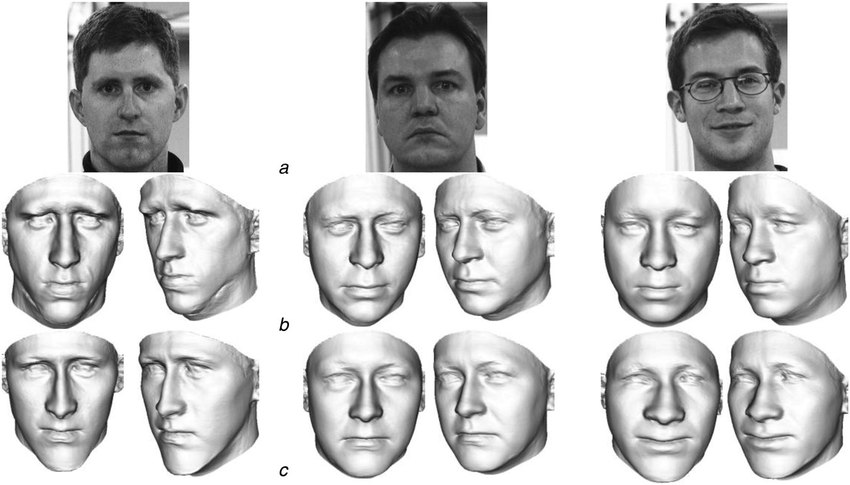
\includegraphics[width=0.8\textwidth]{images/inverse_problem_vision.png}
    \captionof{figure}{Minh họa bài toán nghịch đảo trong Thị giác Máy tính. Quá trình vật lý (thuận) chiếu một cảnh 3D phức tạp lên một mặt phẳng ảnh 2D, làm mất thông tin chiều sâu. Nhiệm vụ của Thị giác Máy tính (nghịch đảo) là suy luận về thế giới 3D từ dữ liệu 2D thiếu thốn.}
    \label{fig:inverse_problem}
\end{center}

Chính sự mơ hồ và thách thức của bài toán nghịch đảo này là động lực thúc đẩy sự phát triển của vô số kỹ thuật, từ hình học, thống kê đến học máy, nhằm đưa ra những giả định hợp lý về thế giới để tìm ra lời giải khả dĩ nhất.

\subsection{Định nghĩa và Phân biệt các Lĩnh vực liên quan}

Để hiểu rõ bản chất của Thị giác Máy tính, điều quan trọng là phải phân biệt nó một cách rạch ròi với các lĩnh vực có liên quan mật thiết nhưng mục tiêu lại khác biệt.

\subsubsection{Thị giác Máy tính (Computer Vision) vs. Xử lý ảnh (Image Processing)}

Đây là sự phân biệt quan trọng nhất. Như đã giới thiệu, Xử lý ảnh tập trung vào các phép biến đổi ảnh-sang-ảnh, trong khi Thị giác Máy tính hướng tới việc biến đổi ảnh-sang-thông tin. Mối quan hệ giữa chúng có thể được xem là cộng sinh: CV thường sử dụng các kỹ thuật của IP như một bước tiền xử lý thiết yếu.

\begin{description}
    \item[Xử lý ảnh (Image Processing):] Tập trung vào việc thao tác trên tín hiệu hình ảnh để tăng cường hoặc sửa đổi nó. Nó hoạt động ở tầng cú pháp (syntactic level) của dữ liệu.
    \begin{itemize}
        \item \textbf{Mục tiêu:} Cải thiện chất lượng (khử nhiễu, làm sắc nét), thay đổi biểu diễn (nén ảnh, biến đổi Fourier), hoặc trích xuất các thuộc tính cấp thấp (phát hiện biên).
        \item \textbf{Ví dụ kinh điển:} Áp dụng bộ lọc Gaussian để làm mờ ảnh, sử dụng phép cân bằng biểu đồ độ sáng (histogram equalization) để tăng độ tương phản.
        \item \textbf{Đầu ra:} Một ma trận pixel khác.
    \end{itemize}
    \item[Thị giác Máy tính (Computer Vision):] Tập trung vào việc diễn giải nội dung của hình ảnh để đưa ra quyết định hoặc xây dựng một mô tả. Nó hoạt động ở tầng ngữ nghĩa (semantic level) của dữ liệu.
    \begin{itemize}
        \item \textbf{Mục tiêu:} Nhận dạng đối tượng, phân loại cảnh, tái tạo cấu trúc 3D, hiểu hành động.
        \item \textbf{Ví dụ kinh điển:} Một hệ thống xe tự lái sử dụng camera để xác định "có một người đi bộ đang băng qua đường ở khoảng cách 20 mét".
        \item \textbf{Đầu ra:} Một biểu diễn trừu tượng, có cấu trúc (vd: nhãn, tọa độ, mô hình 3D).
    \end{itemize}
\end{description}

\subsubsection{Thị giác Máy tính vs. Đồ họa Máy tính (Computer Graphics)}

Nếu CV là bài toán nghịch đảo, thì \textbf{Đồ họa Máy tính (Computer Graphics)} chính là bài toán thuận. Đồ họa máy tính bắt đầu với một mô tả trừu tượng, có cấu trúc của một cảnh (ví dụ: mô hình 3D của các vật thể, vị trí nguồn sáng, thuộc tính vật liệu) và có nhiệm vụ tạo ra (render) một hoặc nhiều hình ảnh 2D chân thực từ mô tả đó. Hai lĩnh vực này là hai mặt của cùng một đồng xu, và sự giao thoa giữa chúng ngày càng trở nên quan trọng, đặc biệt trong việc tạo dữ liệu tổng hợp (synthetic data) để huấn luyện các mô hình CV.

\subsection{Hai Kỷ nguyên của Thị giác Máy tính: Sự Thay đổi Mô hình Nền tảng}

Lịch sử hiện đại của Thị giác Máy tính chứng kiến một sự chuyển dịch mô hình (paradigm shift) rõ rệt, phân chia lĩnh vực này thành hai kỷ nguyên chính dựa trên cách tiếp cận cốt lõi để trích xuất thông tin.

\begin{center}
    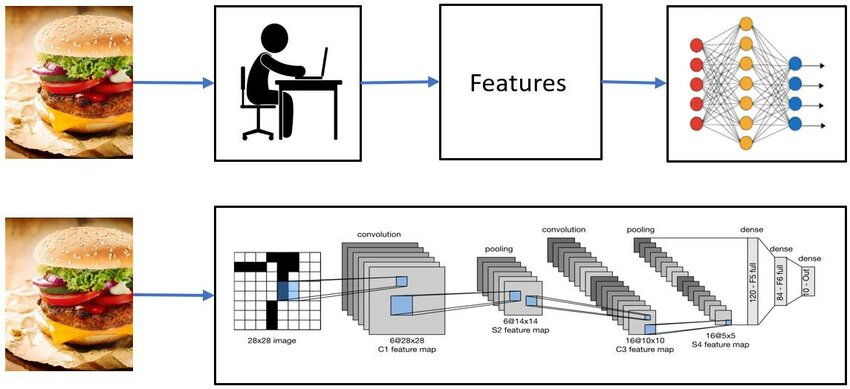
\includegraphics[width=1.0\textwidth]{images/classical_vs_dl_pipeline.png}
    \captionof{figure}{So sánh quy trình làm việc điển hình giữa Thị giác Máy tính cổ điển và hiện đại. Kỷ nguyên cổ điển đòi hỏi sự can thiệp sâu của con người trong việc thiết kế đặc trưng. Kỷ nguyên Học sâu tự động hóa quá trình này thông qua một mô hình end-to-end.}
    \label{fig:classical_vs_dl}
\end{center}

\subsubsection{Kỷ nguyên Cổ điển: Triều đại của Đặc trưng Thủ công (Handcrafted Features)}
\textit{(Trước khoảng năm 2012)}

Trong kỷ nguyên này, quy trình giải quyết một bài toán CV là một chuỗi các bước rời rạc và đòi hỏi sự tinh chỉnh sâu sắc từ các chuyên gia. Trọng tâm của giai đoạn này là việc thiết kế các thuật toán thông minh để trích xuất các \textbf{đặc trưng (features)}—những biểu diễn số nhỏ gọn, bất biến và mang tính thông tin cao của các vùng ảnh.

\begin{description}
    \item[Trực giác:] Các chuyên gia cố gắng mã hóa những hiểu biết của con người về thị giác vào các thuật toán. Ví dụ, để nhận dạng một vật thể, ta cần tìm các điểm đặc biệt (góc, cạnh) không thay đổi khi vật thể bị xoay, thay đổi kích thước hay chiếu sáng.
    \item[Các bộ trích xuất đặc trưng nổi tiếng:]
    \begin{itemize}
    	\item \textbf{\hyperref[subsec:sift]{SIFT (Scale-Invariant Feature Transform)} \cite{Lowe2004}}: Một thuật toán cột mốc, có khả năng phát hiện các "điểm đặc trưng" (keypoints) và tạo ra các vector mô tả (descriptors) có tính bất biến với phép co giãn (scale), xoay (rotation), và thay đổi ánh sáng một phần. Nó đã thống trị nhiều bài toán matching và nhận dạng trong gần một thập kỷ.
    	
    	\item \textbf{\hyperref[subsec:hog]{HOG (Histogram of Oriented Gradients)} \cite{Dalal2005}}: Được phát triển ban đầu cho bài toán phát hiện người đi bộ. Ý tưởng cốt lõi là hình dạng của một đối tượng có thể được biểu diễn tốt bằng sự phân bố của hướng các gradient cường độ sáng. HOG chia ảnh thành các ô nhỏ (cells), tính toán biểu đồ (histogram) của hướng gradient trong mỗi ô, và kết hợp chúng lại để tạo thành một vector đặc trưng duy nhất.
    \end{itemize}
   
    \item[Quy trình làm việc (Pipeline):]
    \begin{enumerate}
        \item \textbf{Tiền xử lý (Preprocessing):} Chuẩn hóa ảnh (thay đổi kích thước, chuyển sang ảnh xám).
        \item \textbf{Trích xuất đặc trưng (Feature Extraction):} Áp dụng một thuật toán được thiết kế thủ công (như SIFT, HOG) để biến ảnh thành một vector đặc trưng có kích thước cố định.
        \item \textbf{Học máy (Machine Learning):} Dùng vector đặc trưng này làm đầu vào cho một mô hình học máy nông (shallow model) như SVM, Logistic Regression, hoặc Random Forest để huấn luyện bộ phân loại.
    \end{enumerate}
    \item[Hạn chế:] Mặc dù đạt được nhiều thành công, cách tiếp cận này có những giới hạn cố hữu. Hiệu năng của toàn bộ hệ thống bị giới hạn bởi chất lượng của bộ trích xuất đặc trưng. Việc thiết kế một bộ đặc trưng tốt cho một bài toán cụ thể là một công việc tốn nhiều công sức, đòi hỏi nhiều thử nghiệm và kiến thức chuyên môn, và thường không thể chuyển giao tốt sang các bài toán khác.
\end{description}

\subsubsection{Kỷ nguyên Học sâu: Cuộc Cách mạng của Đặc trưng Học được (Learned Features)}
\textit{(Từ khoảng năm 2012 đến nay)}

Năm 2012 là một bước ngoặt lịch sử với sự ra đời của AlexNet \cite{Krizhevsky2012}, một Mạng Nơ-ron Tích chập (CNN) sâu đã giành chiến thắng áp đảo trong cuộc thi nhận dạng hình ảnh ImageNet. Sự kiện này đã khởi đầu cho một cuộc cách mạng, thay đổi hoàn toàn cách chúng ta tiếp cận Thị giác Máy tính.

\begin{description}
    \item[Trực giác:] Thay vì nói cho máy tính biết phải tìm kiếm đặc trưng gì, chúng ta thiết kế một kiến trúc mạng đủ lớn và linh hoạt, sau đó cung cấp cho nó một lượng dữ liệu khổng lồ và để nó tự học xem những đặc trưng nào là hữu ích nhất cho tác vụ. Quá trình này được gọi là \textbf{học biểu diễn (representation learning)}.
    \item[Hệ thống phân cấp đặc trưng (Hierarchy of Features):] Một trong những sức mạnh lớn nhất của CNN là khả năng học một cách tự động một hệ thống phân cấp các đặc trưng.
    \begin{itemize}
        \item \textbf{Các lớp đầu (Lower Layers):} Tự động học cách phát hiện các đặc trưng cơ bản, phổ quát như cạnh, góc, và các đốm màu.
        \item \textbf{Các lớp giữa (Mid Layers):} Kết hợp các đặc trưng cấp thấp lại để hình thành các cấu trúc phức tạp hơn như mắt, mũi, tai, hoặc các bộ phận của vật thể.
        \item \textbf{Các lớp cuối (Higher Layers):} Tổ hợp các bộ phận lại để nhận dạng các đối tượng hoặc khái niệm hoàn chỉnh.
    \end{itemize}
    \item[Quy trình làm việc (End-to-End Pipeline):]
    \begin{enumerate}
        \item \textbf{Chuẩn bị dữ liệu:} Thu thập một tập dữ liệu lớn có gán nhãn (ví dụ: hàng triệu ảnh chó và mèo).
        \item \textbf{Huấn luyện End-to-End:} Đưa toàn bộ ảnh thô (ma trận pixel) vào đầu vào của mạng CNN. Mạng sẽ tự động thực hiện cả hai quá trình trích xuất đặc trưng và phân loại. Toàn bộ các tham số của mạng, từ lớp đầu tiên đến lớp cuối cùng, được tối ưu hóa đồng thời thông qua thuật toán lan truyền ngược (backpropagation) để giảm thiểu sai số giữa dự đoán và nhãn thật.
    \end{enumerate}
    \item[Ưu điểm:] Cách tiếp cận này loại bỏ "nút thắt cổ chai" của việc thiết kế đặc trưng thủ công. Nó cho phép các mô hình học được những biểu diễn vô cùng phong phú và phức tạp từ dữ liệu, dẫn đến hiệu năng vượt trội trên hầu hết các bài toán CV. Mô hình trở nên tổng quát hơn, và kỹ năng của kỹ sư chuyển từ "thiết kế thuật toán đặc trưng" sang "thiết kế kiến trúc mạng" và "kỹ thuật huấn luyện".
\end{description}

\subsection{Phạm vi và Phân loại các Bài toán Thị giác Máy tính}

Thị giác Máy tính là một lĩnh vực rộng lớn với một hệ sinh thái các bài toán đa dạng. Chúng có thể được phân loại dựa trên mức độ phức tạp và trừu tượng của thông tin đầu ra, tạo thành một phổ từ nhận thức cấp thấp đến cấp cao.

\begin{figure}[h!]
    \begin{center}
        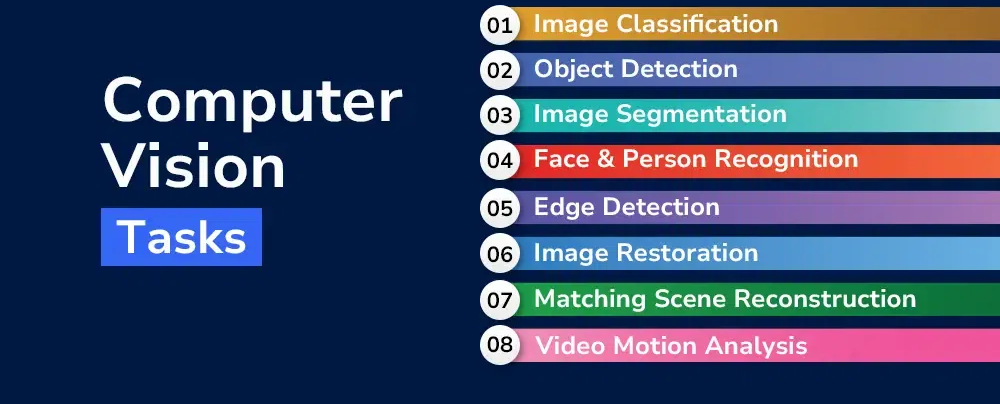
\includegraphics[width=1.0\textwidth]{images/cv_tasks_spectrum_detailed.png}
        \captionof{figure}{Phổ các bài toán trong Thị giác Máy tính. Các tác vụ được sắp xếp theo mức độ trừu tượng tăng dần của đầu ra, từ xử lý pixel cấp thấp đến diễn giải ngữ nghĩa cấp cao của toàn bộ cảnh.}
        \label{fig:cv_tasks_spectrum_detailed}
    \end{center}
\end{figure}

\subsubsection{Thị giác Cấp thấp (Low-level Vision)}
Đây là những tác vụ xử lý gần với đầu vào pixel nhất, thường không liên quan đến ngữ nghĩa.
\begin{itemize}
    \item \textbf{Phục hồi và Nâng cao chất lượng ảnh (Image Restoration \& Enhancement):} Bao gồm các bài toán như siêu phân giải (Super-Resolution), khử nhiễu (Denoising), khử mờ (Deblurring).
    \item \textbf{Xử lý Màu sắc và Tông màu (Color and Tone Processing):} Chuyển đổi màu sắc (Colorization), cân bằng trắng (White Balance), chuyển đổi phong cách (Style Transfer).
\end{itemize}

\subsubsection{Thị giác Cấp trung (Mid-level Vision)}
Các tác vụ này tạo ra các biểu diễn có cấu trúc hơn từ ảnh, làm cầu nối giữa pixel và đối tượng.
\begin{itemize}
    \item \textbf{Phân đoạn Ảnh (Image Segmentation):} Gán một nhãn cho mỗi pixel, phân chia ảnh thành các vùng có ý nghĩa.
        \begin{description}
            \item[Semantic Segmentation:] Phân loại mỗi pixel vào một lớp ngữ nghĩa (vd: đường, xe, trời).
            \item[Instance Segmentation:] Mở rộng từ semantic, phân biệt các thực thể riêng lẻ trong cùng một lớp (vd: xe 1, xe 2).
            \item[Panoptic Segmentation:] Kết hợp cả hai, gán cho mỗi pixel cả nhãn lớp và ID thực thể.
        \end{description}
    \item \textbf{Ước lượng các Thuộc tính Hình học:}
        \begin{description}
            \item[Ước lượng Chiều sâu (Depth Estimation):] Từ ảnh 2D, suy ra bản đồ chiều sâu 3D.
            \item[Ước lượng Bề mặt pháp tuyến (Surface Normal Estimation):] Ước lượng hướng của bề mặt tại mỗi pixel.
            \item[Ước lượng Dòng quang học (Optical Flow Estimation):] Ước lượng vector chuyển động của các pixel giữa hai khung hình video liên tiếp.
        \end{description}
\end{itemize}

\subsubsection{Thị giác Cấp cao (High-level Vision)}
Đây là các tác vụ nhận thức chính, đòi hỏi sự diễn giải ngữ nghĩa sâu sắc.
\begin{itemize}
    \item \textbf{Phân loại (Classification):} Gán một hoặc nhiều nhãn cho toàn bộ ảnh (vd: "phong cảnh", "chân dung").
    \item \textbf{Phát hiện (Detection):} Định vị và phân loại các đối tượng bằng các hộp giới hạn (vd: phát hiện vật thể, phát hiện khuôn mặt).
    \item \textbf{Nhận dạng (Recognition):} Một dạng phân loại chuyên biệt, xác định một thực thể cụ thể (vd: nhận dạng một người nổi tiếng, một địa danh).
    \item \textbf{Ước lượng Tư thế (Pose Estimation):} Xác định vị trí các khớp chính của người hoặc vật thể.
\end{itemize}

\subsubsection{Phân tích Video và Chuỗi ảnh}
Mở rộng các bài toán trên sang chiều thời gian.
\begin{itemize}
    \item \textbf{Theo dõi Vật thể (Object Tracking):} Theo dõi vị trí và ID của một đối tượng qua các khung hình.
    \item \textbf{Nhận dạng Hành động (Action Recognition):} Phân loại hành động đang diễn ra trong một đoạn video (vd: "chạy", "nhảy", "bắt tay").
\end{itemize}

\subsubsection{Thị giác Đa phương thức và Sáng tạo (Multimodal \& Generative Vision)}
Các lĩnh vực tiên tiến, kết hợp thị giác với các phương thức khác (ngôn ngữ, âm thanh) và tạo ra nội dung mới.
\begin{itemize}
    \item \textbf{Mô tả ảnh/video (Image/Video Captioning):} Tự động tạo ra một câu mô tả nội dung.
    \item \textbf{Trả lời câu hỏi bằng hình ảnh (Visual Question Answering - VQA):} Trả lời một câu hỏi dựa trên nội dung của một hình ảnh.
    \item \textbf{Sinh ảnh/video (Image/Video Generation):} Tạo ra nội dung thị giác mới từ văn bản, từ một ảnh khác, hoặc từ nhiễu ngẫu nhiên.
    \item \textbf{Tái tạo 3D từ ảnh (3D Reconstruction from Images):} Xây dựng mô hình 3D từ một hoặc nhiều ảnh 2D, sử dụng các kỹ thuật như NeRF \cite{Mildenhall2020} hay 3D Gaussian Splatting.
\end{itemize}

\section*{Tài liệu tham khảo}
\begin{itemize}
    \item[1] Marr, D. \textit{Vision: A Computational Investigation into the Human Representation and Processing of Visual Information}. MIT Press, 1982.
    \item[2] Forsyth, D. A.; Ponce, J. \textit{Computer Vision: A Modern Approach}. 2nd ed. Pearson, 2012.
    \item[3] Szeliski, R. \textit{Computer Vision: Algorithms and Applications}. 2nd ed. Springer, 2022.
    \item[4] Lowe, D. G. Distinctive Image Features from Scale-Invariant Keypoints. \textit{International Journal of Computer Vision} \textbf{2004}, \textit{60}(2), 91–110.
    \item[5] Dalal, N.; Triggs, B. Histograms of Oriented Gradients for Human Detection. In \textit{Proceedings of the IEEE Conference on Computer Vision and Pattern Recognition (CVPR)}, 2005.
    \item[6] Krizhevsky, A.; Sutskever, I.; Hinton, G. E. ImageNet Classification with Deep Convolutional Neural Networks. In \textit{Proceedings of the Advances in Neural Information Processing Systems (NIPS)}, 2012.
    \item[7] Mildenhall, B., et al. NeRF: Representing Scenes as Neural Radiance Fields for View Synthesis. In \textit{Proceedings of the European Conference on Computer Vision (ECCV)}, 2020.
    \item[8] Trigka, M.; Dritsas, E. A Comprehensive Survey of Deep Learning Approaches in Image Processing. \textit{Sensors} \textbf{2025}, \textit{25}, 531.
    \item[9] Ai, H.; Cao, Z.; Wang, L. A Survey of Representation Learning, Optimization Strategies, and Applications for Omnidirectional Vision. \textit{arXiv preprint arXiv:2502.10444} \textbf{2025}.
\end{itemize}